\begin{jointwork}\label{ch:SimulatingMarketplace}
	In this section we will outline the requirements and challenges of transferring the vast amount of features and parameters that influence vendor and customer decisions in real recommerce markets to our simulated market environment. We will take a brief look at different market scenarios as well as how our customers work, with a focus on the unique feauture of recommerce markets; the buyback of used items by the vendors. The focus of this chapter will however lie on the vendors, the Rule-Based as well as the ones trained using Reinforcement-Learning, comparing their features and how they fare against each other. These comparisons will be done using our various monitoring tools, which will be explained in the following chapter, \nameref{ch:Approaches} and put to use in \nameref{ch:AnalyzingGraphs}. For further information on the whole framework structure, see \cite{LeoThesis}, for detailed insights into our market processes, see \cite{NickThesis}.
\end{jointwork}

\section{Market scenarios}\label{sec:MarketScenarios}

In our framework, we implemented a number of `market blueprints' both for classic Linear Economy markets, as well as for Circular Economy markets both with and without rebuy-prices enabled. There are marketplaces available for each combination of the following two features:
\begin{enumerate}
	\item Marketplace type: Linear Economy, Circular Economy, Circular Economy with rebuy-prices
	\item Market environment: Monopoly, Duopoly, Oligopoly
\end{enumerate}
The marketplace type defines the number of prices the vendor has to set. In a Linear Economy, vendors only set prices for new items, in a Circular Economy prices for refurbished items need to be set as well. In order to simulate a recommerce market, the user can choose a Circular Economy with rebuy-prices. The market environment defines the number of competing vendors in the simulation: Monopolistic and competitive markets are available, where the Duopoly is simply a particular version of an Oligopoly. Depending on the chosen market environment, one, two, or any number of vendors can be chosen to be used in the experiment. \Cref{fig:OverviewDiagram} shows a reduced overview of the classes in our framework which concern themselves with the market simulation, and how they interact with each other during the simulation.

In the most common usecase of our framework, the training of Reinforcement-Learning agents, only the agent (or multiple agents in the case of training multiple Reinforcement-Learning agents against each other) that is to be trained needs to be configured by the user, as each market environment is equipped with a pre-defined set of competitors that will play against the agent defined by the user. To allow for more control over the simulation, users are however also able to change these competitors to use any vendors they want - as long as they are a valid fit for the marketplace type and the number of competitors chosen matches the market environment.

\begin{figure}[t]
	\centering
	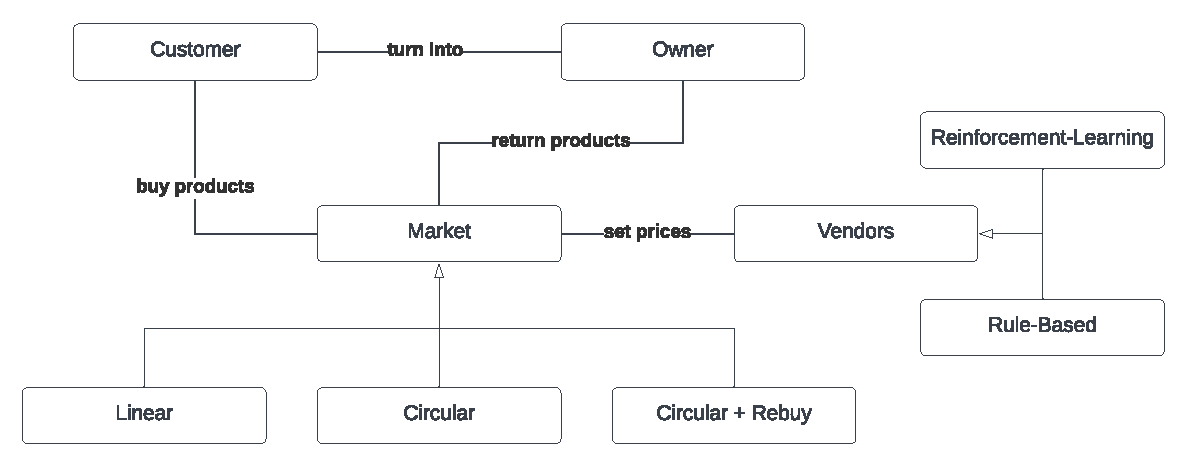
\includegraphics[width = \textwidth]{images/overview_diagram.pdf}\\
	\caption{Class diagram outlining interactions between classes concerning the market simulation.}\label{fig:OverviewDiagram}
\end{figure}

\section{Customers}\label{sec:Customers}

Customers are at the center of every type of marketplace, which makes them an integral part of our market simulation. However, since each customer in the real market is an individual with different reasonings and makes purchase decisions based upon personal preferences, modelling a realistic depiction of real-world customers proves to be very difficult and time-consuming. For this reason we decided to keep our initial implementation of the customers as simple as possible, taking into account future extension and scalability concerns.

Most customers' behaviour can be classified into one of a (non-exhaustive) number of categories, such as \emph{Perfectionistic} or \emph{Impsulsive} consumers, proposed in~\cite{ShoppingStyles} (also see \Cref{tab:shoppingStyles}). As we are focussing on dynamic pricing and our vendors can only change/influence the prices of their products, we decided on primarily building customers that value price over any other features a product may have, thereby incentivizing our vendors to make the most of their pricing power. This behaviour coincides with the shopping style of the \emph{Price Conscious} or\emph{Value for money} consumer.

\todo{I could remove this next paragraph, since we focus on Circular Economies}To make Linear markets a little more complex and add another dimension than just the \emph{new price} of a product for vendors to consider, random quality values are assigned to each vendor's products. Customers in this economy model were modelled take this quality value into account when making their purchasing decisions, further reinforcing the shopping style mentioned above. As Circular Economy markets are inherently more complex than their linear counterparts (through the addition of two new price channels, which influence each other through their effect on customers), it was decided to remove the additional layer of quality values from these markets.

Within each simulated step, after the various vendors have set their prices, purchase decisions are made by the customers. To save on computational time, probability distributions are used to determine what part of the total number of customers will decide to take which action. See below for the way these distributions are calculated for an exemplary Circular Economy marketplace, for further information also see \cite{NickThesis}.

\begin{definition}\label{def:customerDecisions}
	Let \(P_{in}\) be the price of the new and \(P_{ir}\) the price of the refurbished product of vendor \(i\). Using these prices, for each vendor, we define \(R_{in}\) as the \emph{preference ratio} regarding \(P_{in}\):
	\[
		R_{in} := \frac{10}{P_{in}} - e^{P_{in} - 8}
	\]
	and similarly, \(R_{ir}\) as the \emph{preference ratio} regarding \(P_{ir}\):
	\[
		R_{ir} := \frac{5.5}{P_{ir}} - e^{P_{ir} - 5}
	\]
\end{definition}\todo{Graph for the preference ratios in Appendix?}

In order to be usable as a probability distribution, the different ratios need to add up to \(1\). We use \emph{softmax} to normalize our values, after which each \emph{preference ratio} will be within the interval \((0,1)\), with all ratios adding up to \(1\) as needed.

Following this, the market uses a \emph{multinomial} distribution to draw \(n\) samples, with \(n\) being the number of customers making a pruchasing decision in this step of the simulation.

As mentioned above, the current decisionmaking process of customers in our simulation is still quite basic. \fullref{sec:DivergingFromRealMarket} introduces a number of parameters and circumstances that can be used to make customer behaviour more realistic. Through the modular approach when building the framework, any customer behaviour implemented in the future can easily be added to the pool of available options, as long as it manifests in the form of a probability distribution, at which point the number of customers can be split between different distributions when drawing from the \emph{multinomial} distribution (or any other distribution if so desired).

\subsection*{Owners}

Once a customer has decided to buy a product from any of the available vendors, they turn into an \emph{owner}. In the next step of the simulation, they are offered the option of selling their now used product back to one of the vendors. If they decide to do so, the vendor pays them the advertised \emph{re-buy price} and adds the used product to their inventory, from where it can then be sold as a refurbished product in the next step.

In our simulation, all owners are memoryless, meaning that they do not remember the original price they paid for the product. Additionally, each vendor in the market is obligated to buy back any product, independent of the original vendor. In each step, every owner has the option to either keep the product for another step, discard it (meaning it is removed from circulation and not sold back to a vendor), or sell it to any one of the vendors in the market. Similarly to the way we compute customer purchasing decisions, the decisions owners take are also represented through probability distributions. When deciding if and to which vendor a product should be sold, the following formula is used:

\begin{definition}\label{def:ownerDecisions}
	We keep the variables defined in \Cref{def:customerDecisions}. Additionally, let \(P_{ib}\) be the price at which vendor \(i\) is willing to buy back an owner's product. For each vendor, we define \(P_{im}\) as the purchase option with the lowest price:
	\[
		P_{im} := \min(P_{in}, P_{ir})
	\]
	We define the likelihood \(R_{ib}\) that the owner will return their product to vendor \(i\) as follows:
	\[
		R_{ib} := 2 \cdot e^{(P_{ib} - P_{im}) / P_{im}}
	\]
	Additionally, the owner's \emph{discard preference} \(R_{d}\) is updated for each vendor as follows:
	\[
		R_{d} := \min({R_{d}, \frac{2}{P_{ib}+1}})
	\]
	Meaning the owner is more likely to discard their product if re-buy prices are low across the board.
\end{definition}

\section{Vendors}\label{sec:ExplainVendors}

Vendors are the main focus of our market simulation. While our framework will not be able to reproduce all types of pricing models used in the real market, we strive to model as many different models as possible (and feasable in the scope of the project). Due to the modular nature of the framework, it is possible for users to easily create and add their own pricing strategies in the form of a vendor that can play on a market. This allows users to not only add other Reinforcement-Learning algorithms, but also to define new Rule-Based strategies. For this reason, we also do not restrict the usage of our monitoring tools to just Reinforcement-Learning agents, but allow users to monitor any combination of vendors.\todo{Do I need to further motivate \emph{why} we allow this?}

We will use four types of dynamic pricing models, as defined in `Dynamic pricing models for electronic business'~\cite{dynamicPricingModels}, to describe the different models we implemented in our framework. These categories are not mutually exclusive, and many agents belong to more than one category.

\subsection*{Inventory-based models}\label{subsec:InventoryBasedModels}

These are pricing models which are based on inventory levels and similar parameters, such as the number of items in circulation (items which are currently in use by customers). In our framework, almost all Rule-Based agents consider their inventory levels when deciding which prices to set. The only exception to this rule are the simplest of our agents, the \emph{FixedPriceAgents}, which will always set the same prices, no matter the current market state and competitor actions. The prices these agents will set are pre-determined through the user's configuration of the experiment, and will not change over the course of the market simulation.

Inventory-based models are comparatively easy to implement, as they only depend on data immediately available to the vendor. This has the advantage that Rule-Based agents which fall into this category are relatively simple to create and modify. Examples of \emph{Inventory-based agents} in our framework can be found in the \emph{RuleBasedCEAgent}\todo{Compare this agent with other agents, RL, FixedPrice, better Rule-Based!}, one of the first Rule-Based agents we created. This agent does not take pricing decisions of its competitors in the market into account, but simply acts according to its own storage costs, always trying to keep a balance between having enough (refurbished) products to sell back to customers and keeping storage costs low. It does this by checking into which of four possible ranges the current number of stored products falls. The more products the agent already has in storage, the lower it sets the rebuy price (to `prevent' customers from returning more products), and the lower it sets the price for refurbished products, to empty the storage more quickly and prevent high storage costs. While its performance is not necessarily bad, it is still one of the weakest competitors currently available in the framework. For the full implementation logic of the agent's policy, see \Cref{fig:PolicyRuleBasedCE}.

\subsection*{Data-driven models}\label{subsec:DataDrivenModels}

\emph{Data-driven} models take dynamic pricing decisionmaking one level further. They utilize their knowledge of the market, such as customer preferences, past sales data or competitor prices, to derive optimal pricing decisions. Aside from the aforementioned \emph{FixedPriceAgents} and the basic \emph{RuleBasedCEAgent}, all of our other Rule-Based agents fall into this category. One of the most prominent examples of a \emph{Data-driven model} is the \emph{RuleBasedCERebuyAgentCompetitive}, an agent whose basic goal is to always try and undercut competititor prices, while also keeping track of the current amount of items in storage. In its policy, this agent first always undercuts the new price of all other competitors. Then, similar to the \emph{RuleBasedCEAgent}, the agent looks at the current amount of stored products and depending on the range, sets lower prices for refurbished items and higher rebuy-prices, while always trying to give customers a better deal than any of the competitors. Again, the full implementation logic of this vendor's policy is available in the Appendix, under \Cref{fig:PolicyRuleBasedCompetitive}.

Notably, all of our \emph{Data-driven models} are also \emph{Inventory-based} to a certain extent, as handling storage plays a big part in a Circular Economy market setting, where used products need to be bought back from customers and subsequently undergo refurbishment while in inventory of the company. \emph{Data-driven models} have proven to be the most competent Rule-Based agents in our recommerce market scenario, in particular the above described \emph{RuleBasedCERebuyAgentCompetitive}, which is able to outperform most other Rule-Based agents, both \emph{Inventory-based} and \emph{Data-driven models}\todo{Graphs to prove it, use one from Oligopoly experiment?}.

\subsection*{Game theory models}\label{subsec:GameTheory}\todo{If any section needs to be removed here (e.g. for page length), this should be the one}

Game theory concerns itself with the study of models for conflict and cooperation between rational, intelligent entities~\cite{GameTheory}. It is therefore often applicable in situations where competing individuals, acting rationally and selfishly, interact with each other. In our framework, most competitors in the market are influenced in their decisionmaking processes by the actions of other participants of the scenario. This is especially true for the Reinforcement-Learning agents, which base their policy on the received market states, which include their competitor's actions. While none of our Rule-Based agents have been specifically designed to act according to game theoretic strategies, due to the fact that almost all of them consider their competitors prices in their pricing decision, and due to the nature of Reinforcement-Learning trying to maximize their own profits without regard to their competitors performance, behaviour according to Game theory can sometimes be observed. This can be observed especially well in the beginning of training sessions, where Rule-Based competitors often struggle to achieve high profits while the Reinforcement-Learning agent is making great losses, but are then able to increase their profits as the trained agent starts to make better decisions as well. Many examples of such behaviour can be found in the diagrams shown in \fullref{ch:AnalyzingGraphs}, such as in \Cref{fig:SACDuopolyProfitsMean}.

During training, Reinforcement-Learning agents observe the market state, which includes prices and sales data not only of themselves but also the other vendors in the market. Using this data, the algorithms try to predict how their prices will influence customer behaviour as well as the competing vendors. In some cases, depending on the concrete behaviour of the competitors, vendors may cooperate in driving prices higher together, in other cases the agents may act seemingly irrationally, lowering prices in order to force their opponents to lower theirs as well. An example of such behaviour can be seen in the development of prices for new items set by the two competing vendors in \Cref{fig:SACDuopolyMixedGraphs4}.

\subsection*{Machine learning models}\label{subsec:MachineLearningModels}

All of our Reinforcement-Learning agents fall into this category. As they are not the focus of this thesis, we will not go into detailed explanations of the various models used. The following will give a short overview over the different algorithms used in our framework.

There are two `origins' of the algorithms in our framework. In the earlier phases, \hyperref[item:QLearning]{Q-Learning} and \hyperref[item:ActorCritic]{Actor-Critic} algorithms were custom implemented by us. Later on, we used the \hyperref[item:StableBaselines]{Stable-Baselines} library to incorporate a greater number of pre-implemented algorithms into our framework. While these are not as easily configurable, they can quickly be used without much additional work.

\begin{itemize}
	\item \phantomsection\emph{Q-Learning}:\label{item:QLearning} \emph{Q-Learning} agents were the first Reinforcement-Learning agents we introduced in our framework, as its algorithm is one of the easier ones to implement~\cite{reinforcementLearningOverview}. The \emph{Q-Learning} algorithm used in our framework is implemented using the \emph{pytorch} framework (see \cite{Pytorch}). However, the drawback of using \emph{Q-Learning} in our framework is that it can only be applied to discrete action and state spaces. This means that when using \emph{Q-Learning}, only `whole' prices can be set by our vendors, and any decimal places must be omitted. This of course limits the framework in its realism, as the fine-tuning of prices using decimal places can be critical in influencing customer decisions. In the initial exploration-phase of our simulation framework this was not a problem, as relatively small action spaces were used, adapted to this limitation. Even now, our simulation framework still operates on discrete action and state spaces, both to allow algorithms like \emph{Q-Learning} to still function and to not overly complicate the simulation, as many of the other components (such as customer behaviour, see \nameref{sec:Customers}) are still very basic in their nature as well. While approaches for \emph{Q-Learning} algorithms that can work with continuous action and state spaces have been presented in the past (\cite{QLearningContinuous},~\cite{QLearningContinuous2}), we have chosen not to implement such an algorithm in our framework, but rather explore approaches other than \emph{Q-Learning}, such as \emph{Actor-Critic} algorithms, introduced below.

	\item \phantomsection\emph{Actor-Critic}:\label{item:ActorCritic} \emph{Actor-Critic} algorithms are more complex than Q-Learning algorithms, and have therefore been implemented later in the process. They are structured different then Q-Learning algorithms in the way that they are `split' into two parts: The \emph{actor} is responsible for selecting actions, while the \emph{critic} is responsible for critizing the actions taken by the \emph{actor}, thereby improving its performance~\cite{ActorCritic}. Similar to the \emph{Q-Learning} agents, the \emph{Actor-Critic} algorithms have also been implemented by us. In total, one discrete and two continuous \emph{Actor-Critic} agents can be used, in addition to those provided through \emph{Stable-Baselines}, see the next section.

	\item \phantomsection\emph{Stable-Baselines}:\label{item:StableBaselines} Stable-Baselines provides a number of open-source implementations for various Reinforcement-Learning algorithms. In our framework, we use the latest version of these algorithms, through \emph{Stable-Baselines3} \cite{StableBaselines3}. The advantage when using algorithms provided through Stable-Baselines lies in the fact that they need close to no custom implementation from our end, we can instead interact with them through very simple interfaces. This cuts down on the amount of time and effort that needs to be spent developing, implementing and maintaining these powerful algorithms, and allows us to introduce a higher number of algorithms than would otherwise be possible. Currently, five different \emph{Stable-Baselines3} algorithms are used in our simulation framework, see the \emph{Stable-Baselines3} documentation~\cite{StableBaselines3Algorithms} and the referenced papers for more information about the different algorithms:
	      \begin{itemize}
		      \item \emph{A2C}: Advantage-Actor-Critic (\cite{StableBaselines3A2C})
		      \item \emph{DDPG}: Deep deterministic policy gradient (\cite{StableBaselines3DDPG})
		      \item \emph{PPO}: Proximal Policy Optimization (\cite{StableBaselines3PPO})
		      \item \emph{SAC}: Soft Actor-Critic (\cite{StableBaselines3SAC})
		      \item \emph{TD3}: Twin-delayed deep deterministic policy gradient (\cite{StableBaselines3TD3})
	      \end{itemize}
	      We will be using some of these algorithms in our experiments and briefly compare them with our Rule-Based approaches using our various monitoring tools, which are introduced in \nameref{ch:Approaches}.
\end{itemize}
